\documentclass[11pt,a4paper]{article}
\usepackage{fontspec}
\usepackage[margin=25mm]{geometry}
\usepackage{amsmath,amssymb,booktabs,array,graphicx}
\usepackage{microtype}
\usepackage[hidelinks]{hyperref}
\usepackage{xurl}
\setlength{\emergencystretch}{2em}
\newcommand{\Wall}{81.959}
\newcommand{\CPU}{81.472}
\newcommand{\RSS}{273.05}
\newcommand{\Output}{84.65}
\newcommand{\CandidateThreshold}{40.81854}
\newcommand{\RelativeIncrease}{13.30}

\title{When Should a Digital-Twin Alarm Clear?\\Recovery Evidence under Motion-Model Mismatch}
\author{Muhammad Usman \and Haiqa Mushtaq}
\date{17 October 2026}
\begin{document}
\maketitle
\begin{abstract}
A small prediction error does not necessarily mean that a disturbed robot has returned to its intended motion. We examine alarm recovery using a corrected motion observer and a separate reference driven by approved commands. The alarm clears only after measured joint state remains within a reference tolerance, including a noise margin, for ten consecutive samples. We compare this fixed-return rule with autoregressive predictors, rolling means, CUSUM, hysteresis, command resets and component ablations. The evaluation comprises 144 simulated episodes with multisine and chirp commands, varied plant parameters, actuator lag and sensor noise. All configurations and thresholds were fixed before generating the evaluation data. Across 90 interventions, fixed return had no premature clears under the specified recovery criterion. It nevertheless alarmed on 2,778 of 59,400 benign observations, compared with 2,452 for fused hysteresis, and failed the predeclared improvement criterion. At the same entry threshold, removing the ten-sample dwell caused premature clearing in 44 events. Removing reference-based alarm entry changed no decision. The dwell therefore improved recovery behavior at the cost of additional benign alarm time. These results support evaluating alarm onset and recovery separately. Their scope is limited to the simulated dynamics and the assumption of protected commands and truthful sensing.
\end{abstract}
\noindent\textbf{Keywords:} digital twin; robotic motion; anomaly detection; alarm recovery; model mismatch; cybersecurity; simulation.
\section{Introduction}
An alarm in a robotic system must identify a deviation and remain active for as long as the monitored condition warrants it. These decisions need different evidence. A predictor that follows recent measurements may produce a small error while the robot is still displaced from its approved trajectory. A fixed reference can expose that displacement, but errors in its plant model can also cause alarms during legitimate motion.

We study whether a separate return criterion can preserve alarm evidence through recovery without increasing alarms during authorized command changes. A following observer supplies a prediction error for alarm entry. A reference driven by the approved command supplies the return condition. Once triggered, the alarm clears only after the measured state stays close to this reference for ten consecutive samples.

We evaluate this rule on 144 simulated episodes and compare 23 methods and ablations. All context-aware methods receive the same protected commands and noisy joint observations. Two comparisons separate the effects of calibration and recovery logic: one calibrates each complete decision rule on the same normal data, while the other holds the entry threshold fixed. The experiment tests an engineering combination of established components; it makes no claim of algorithmic originality.

\section{Related work}
CASPER detects motion anomalies using external inertial measurements from a robotic arm and evaluates deviations introduced through joint-velocity changes \cite{casper}. Its successor investigates real-time detection on edge hardware \cite{edge}. Both concern movement monitoring, but their external-IMU inputs differ from the four joint-state channels and protected commands used here. Their published results therefore cannot be compared directly with this simulation.

TWINE combines a manufacturing digital twin with explainable anomaly detection \cite{twine}. Its supervised classification workflow uses labels that are unavailable to our normal-only procedure. Ayankoso et al. combine trajectory-change recognition with condition monitoring \cite{ayankoso}. Recognizing a changed trajectory is relevant to legitimate operation, although the movement alone does not establish whether a command was authorized.

Observer-based fault diagnosis already addresses the effects of gain and model uncertainty on detection \cite{meseguer}. CUSUM accumulates evidence of persistent changes \cite{nist}. More recent work examines adaptive interval observers for actuator faults \cite{rapio} and digital-twin-based false-data-injection detection in robotic vehicles \cite{kaisar}. Full-method comparisons with these two recent studies remain unresolved because complete manuscripts or implementation details were unavailable in the source audit.

Our executable comparisons use specified predictors and classical alarm rules under common information access. The earlier nine-channel IMU predictors remain a separate experiment. No published detector's complete experimental protocol has been reproduced in the present study.

\section{Virtual plant, information and threat model}
The simulated plant is a horizontal two-revolute-joint arm with point masses. Its state is $x=[q_1,q_2,\dot q_1,\dot q_2]^\top$, with angles in radians and time in seconds. Writing $a=m_2l_1l_2$ and $d=m_2l_2^2$, the mechanical equations are
\begin{align}
 M(q)\ddot q+c(q,\dot q)+B\dot q&=\tau,\\
 M(q)&=\begin{bmatrix}
 (m_1+m_2)l_1^2+d+2a\cos q_2 & d+a\cos q_2\\
 d+a\cos q_2 & d
 \end{bmatrix},\\
 c(q,\dot q)&=a\sin q_2\begin{bmatrix}-2\dot q_1\dot q_2-\dot q_2^2\\\dot q_1^2\end{bmatrix}.
\end{align}
Nominal parameters are $m_1=1$, $m_2=0.8$ kg, $l_1=0.5$, $l_2=0.4$ m and $B=\operatorname{diag}(0.08,0.06)$. A saturated proportional--derivative controller requests
\begin{equation}
 \tau^*=\operatorname{clip}\{K_p(q^c-q)+K_d(\dot q^c-\dot q),-20,20\},
\end{equation}
componentwise, with $K_p=\operatorname{diag}(18,12)$ and $K_d=\operatorname{diag}(4,3)$. For a lagged plant, actuator torque is an additional two-dimensional state satisfying $\dot\tau=(\tau^*-\tau)/T_a$. The zero-lag plant applies $\tau^*$ directly. The monitor retains the lag-free nominal model in every condition. Gravity, contact, flexible links, thermal effects, communication jitter and actuator faults beyond the declared command manipulations are absent.

The plant receives an executed command $u^e=[q^c,\dot q^c]$. The monitor receives a protected approved command $u^a$, a context-validity flag and noisy truthful joint measurements $y=x+\epsilon$. Nominal independent Gaussian sensor standard deviations are $(0.0005,0.0005,0.002,0.002)$. Plant-specific noise scaling is stated below. The attacker changes the downstream executed command without changing the protected approved record or measurement stream. Authorized changes update both command paths. This separates the effect of permission context from the physical shape of a change. Authentication itself is assumed, not implemented or demonstrated.

The detector API excludes executed commands, true states, actual plant parameters, scenario names, intervention schedules and labels. When context is unavailable, the command channel holds its last available value. Context-dependent decisions become unknown. A stateful alarm remains internally latched and its recovery counter resets; unknown observations do not become known negatives. Context-free persistence and AR remain available. The attack model excludes coordinated compromise of the protected command and all sensing channels. The experiment cannot establish security under that stronger adversary or distinguish every mechanical fault from malicious intent.

\section{Prediction and recovery mechanisms}
Let $F_0$ be one nominal integration step and $r_t$ a reference driven by the available approved command. A following observer maintains a separate estimate $\hat x_t^-$. Its recursion is
\begin{align}
 r_{t+1}&=F_0(r_t,u_t^a),\\
 \hat x_{t+1}^-&=F_0\{\hat x_t^-+L(y_t-\hat x_t^-),u_t^a\},
 \qquad L=\operatorname{diag}(0.65,0.65,0.35,0.35).
\end{align}
Scores at $t$ use $\hat x_t^-$ before the current measurement corrects the state. Both trajectories begin at the declared task's initial pose and zero velocity. Parameters, gains and residual scales remain fixed throughout an episode. The observer is synchronized with measurements, while the reference remains driven by approved commands.

With training standard deviation vector $s$, define
\begin{equation}
 e_t^f=\tfrac14\sum_{j=1}^{4}[(y_{t,j}-\hat x^-_{t,j})/s_j]^2,
 \qquad
 e_t^r=\tfrac14\sum_{j=1}^{4}[(y_{t,j}-r_{t,j})/s_j]^2.
\end{equation}
Training means $\bar e^f,\bar e^r$ normalize a fused entry score
\begin{equation}
 z_t=\max(e_t^f/\bar e^f,e_t^r/\bar e^r).
\end{equation}
Ordinary fused hysteresis enters when $z_t>h$ and clears after ten valid consecutive samples at $z_t\le h/2$. An above-threshold observation has priority and restarts the recovery count. 

The fixed-return candidate uses the same entry score but replaces the low-score condition by
\begin{equation}\label{eq:return}
 R_t=\mathbf 1\!\left\{\forall j:\ |y_{t,j}-r_{t,j}|+3\sigma_j\le0.1s_j\right\}.
\end{equation}
After entry, the candidate clears when $R_t=1$ for ten consecutive valid observations without a new entry. The ten-observation window spans nine sample intervals; we report the count explicitly rather than calling it an exact 0.20 s residence time. The $3\sigma$ allowance is a design margin, not a deterministic bound on Gaussian noise or a confidence certificate. In the noisy fresh plant the detector still uses its original nominal $\sigma$.

The saved AR(4) and ARX(4) controls predict standardized state using four preceding observations; ARX also receives the preceding approved command. They use ridge coefficient $0.001$ with an unpenalized intercept. Persistence uses the preceding observation. Their scores are channel-mean squared standardized errors. A 45-sample trailing mean and a CUSUM operate on following-observer error. The latter obeys
\begin{equation}
 C_t=\max\{0,C_{t-1}+\min(e_t^f/\bar e^f,25)-1.5\}.
\end{equation}
The cap and drift remain fixed throughout evaluation.

Additional controls include mode-conditioned fusion, an envelope from three nominal-model parameter combinations, and their ordinary or fixed-return decisions. The envelope score is the maximum per-channel excess outside the sampled trajectory range divided by nominal sensor noise. Mode conditioning uses protected command increments to flag a 50-sample transition interval and fixed training normalizers. A command-reset control clears ordinary fused hysteresis at the start of a detected command-mode interval, before applying the current entry rule; it never receives an intervention boundary.

Six added normal-calibrated variants remove the dwell, remove the noise margin, use reference-only entry, use following-only entry, add following-error hysteresis, or apply the command reset. Removing reference entry retains the reference in the return test. Four further ablations retain the candidate's identical $h$ while changing only its decision rule to point thresholding, ordinary hysteresis, one-sample return or zero-margin return. This second track isolates the return mechanism; its members need not have the same calibration alarm burden. All 23 definitions and exact thresholds are retained in the code and appendix.

\section{Experimental design}
\subsection{Development, calibration and fresh conditions}
Earlier simulation cycles were exposed development evidence. The immediately preceding cycle tested 144 episodes with thirteen methods. Its envelope candidate missed the complete predeclared improvement target and showed substantial extrapolation failure. A simpler fixed-return ablation was the stronger within-range development lead. We selected that ablation before generating the present data; no finding from this cycle selected its configuration.

All fitted coefficients, channel transforms, residual means and mode normalizers were retained from the earlier normal-only study. Eighteen normal calibration episodes provide 16,200 eligible targets. The first thirteen methods retain their exact saved thresholds. Each of six new normal-calibrated methods selects the smallest observed score-grid threshold, including zero and warmup scores, yielding at most 162 eligible normal alarms under its complete decision state machine. Alarms use strict exceedance. The four matched-entry diagnostics instead inherit the candidate threshold, $h=\CandidateThreshold$, without recalibration. The candidate produced 153 calibration alarms; the matched point, hysteresis, no-dwell and no-margin variants produced 4, 65, 44 and 72, respectively. Equal entry thresholds and equal alarm budgets are different experimental controls.

The fresh matrix reserves two analytic tasks. For phase $\theta(s)$, amplitudes $a_1,a_2$ and offset $\phi$, desired positions are
\begin{equation}
 q_1^c=a_1\sin\theta+0.06\sin2\theta,\qquad
 q_2^c=a_2\sin(\theta+\phi)+0.04\sin3\theta.
\end{equation}
Task C uses $\theta=0.75s+0.10\sin(0.2s)$, amplitudes $(0.28,0.38)$ and $\phi=0.55$. Task D uses $\theta=0.45s+0.0125s^2$, amplitudes $(0.33,0.42)$ and $\phi=1.05$. Velocities are analytic derivatives multiplied by the current time-warp rate. Slow commands integrate rate $0.5$ causally. An authorized slowdown retains its accrued phase delay; an unauthorized slowdown rejoins the original approved schedule when command corruption ends. That restoration can create a command discontinuity, which is part of the specified model.

\begin{table}[htbp]\centering\small
\caption{Fresh actual plants. Factors multiply nominal parameters; the monitor is unchanged.}
\begin{tabular}{lcccr}\toprule
Plant & Mass factors $(m_1,m_2)$ & Damping factors & Lag (s) & Noise factor\\\midrule
P1 & $(0.92,1.08)$ & $(1.4,0.7)$ & 0 & 1.0\\
P2 & $(1.18,0.90)$ & $(0.7,1.3)$ & 0.04 & 1.0\\
P3 & $(0.82,1.22)$ & $(1.5,0.6)$ & 0.08 & 1.5\\\bottomrule
\end{tabular}\label{tab:plants}
\end{table}

Each task--plant pair receives noise seeds 17, 42 and 2026, offset by a fixed task/plant formula before generation. Noise is paired across conditions. Eight conditions comprise unchanged motion, authorized offset, authorized slowdown, brief unauthorized offset, persistent unauthorized offset, hold, unauthorized slowdown and an offset with missing command context. Offset magnitude is $-0.18$ rad on joint 1. Interventions start at sample 350; the brief one lasts eight samples (0.16 s), while others end before sample 550. Missing context occupies samples 350--409. Each episode has 1,200 samples at 50 Hz, with the first 100 processed but excluded from metrics. State resets only between independent simulated episodes, never at labels.

The total is $2\times3\times3\times8=144$ episodes, 158,400 eligible observations per method, 59,400 observations in wholly benign episodes and 90 intervention events. These are paired virtual conditions, not 144 independent robots. The two new motion families and torque lag provide a prospective within-simulator challenge beyond new noise seeds, but not independent physical validation. No inferential population confidence interval or seed-based significance claim is made.

\subsection{Metrics and primary criterion}
Point precision, recall and F1 use the scheduled command-corruption labels without point adjustment. Unknown decisions do not count as alarms; their positive labels remain false negatives. Average precision uses underlying scores, with unknown scores ranked below all valid scores and all positive labels retained. Consequently AP evaluates score ranking rather than the complete alarm latch. Variants sharing a score have identical AP even when their alarms differ.

Benign alarm fractions use wholly benign episodes, separating legitimate-operation burden from post-corruption recovery. Alarm episodes per eligible hour count causal rising edges; missing-context reappearance is not a fresh onset. Event overlap means at least one known alarm within the intervention. A fresh detection additionally requires a known alarm rising edge. All misses remain in event denominators; delays are conditional on the stated detected subset. An overlapping alarm alone is not proof of timely new detection.

For evaluation only, physical return is the first start of ten consecutive true-state observations within $0.1s_j$ of the nominal reference in every channel after the executed command is restored, searched within five seconds. This compares simulated state to a modeled trajectory; it is neither a damage metric nor a safety criterion. Premature clearing means an alarm falls after its first known event hit but before that declared return. Unalarmed gaps and absence of return are also preserved. Clearing delay is the first known non-alarm at or after return, up to five seconds. A method that cleared too early can therefore have zero delay: the premature-clear metric must be read alongside it.

The primary criterion requires the candidate to reduce benign alarm points by at least 25\% against \emph{both} fused hysteresis and mode-conditioned hysteresis, without more benign alarm episodes, missed overlaps, missed fresh onsets or premature-clear events. At least 95\% of detected events with a physical return must clear within five seconds. The complete conjunction was specified before generation. Subgroups and component comparisons are descriptive; they do not replace this primary outcome.

\subsection{Implementation and validation}
The configuration, fitted models and calibration thresholds were fixed before evaluation. All methods were scored before outcomes were examined. Fourteen synthetic tests covered command derivatives, lag dynamics, integration refinement, causality, missing-context behavior and threshold rules. Post-run checks verified source and artifact hashes, score replay, state transitions and contingency counts. These checks establish software consistency within the implementation.

The run used an isolated Python 3.12.15/NumPy 1.26.4 environment on an Apple M5 Pro computer with 24 GiB memory. Resource limits were 600 s wall time, 300 s CPU, 1 GiB monitored memory and 160 MiB outputs. No new neural training was performed. Figures and tables were computed from saved results with Python and Matplotlib. AI assistance in study design, implementation and analysis is disclosed in the declarations.

\section{Results}
\subsection{Detection and alarm burden}
The primary improvement criterion failed. Fixed return alarmed on 2,778 benign observations (4.68\%), compared with 2,452 (4.13\%) for fused hysteresis: a \RelativeIncrease\% increase rather than the required reduction. It reduced benign points by 59.41\% against mode hysteresis, which was insufficient because the criterion required improvement against both controls. The candidate had 41 benign alarm episodes versus 45 for fused hysteresis and 175 for mode hysteresis. Its longer alarm time therefore did not imply more alarm episodes.

\begin{table}[htbp]\centering\small
\caption{Selected controls and candidate on the fresh pooled population. Overlap/fresh counts have denominator 90; early denotes events with premature clearing. Full roster appears in Appendix~\ref{app:all}.}
\begin{tabular}{lrrrr}
\toprule
Method & Benign (\%) & F1 & Overlap/fresh & Early \\
\midrule
ARX(4) & 6.00 & 0.644 & 90/80 & 90 \\
Rolling mean (45) & 4.43 & 0.709 & 90/72 & 87 \\
CUSUM & 44.05 & 0.216 & 81/39 & 0 \\
Following hysteresis & 2.57 & 0.795 & 90/72 & 90 \\
Fused hysteresis & 4.13 & 0.677 & 90/72 & 3 \\
Mode hysteresis & 11.52 & 0.519 & 90/72 & 0 \\
Fixed return & 4.68 & 0.650 & 90/72 & 0 \\
\bottomrule
\end{tabular}
\label{tab:main}
\end{table}

Fixed return, fused hysteresis and mode hysteresis each overlapped all 90 events and produced 72 fresh event onsets. All 18 absent fresh onsets for fixed return occurred in the missing-context condition; later known overlap did not satisfy the stricter fresh-onset definition. The candidate had no premature clears or known unalarmed gaps before declared return. Fused hysteresis had premature clearing in three events and 15 gap observations. All 90 candidate events returned and cleared within five seconds; the maximum measured clearing delay was 0.92 s. 

Following-error hysteresis had fewer benign alarms and higher command-interval F1: F1 was 0.795, versus 0.650 for fixed return, with 1,529 benign alarm points. It nevertheless cleared before declared physical return in all 90 events. Its zero maximum clearing delay reflects alarms already absent at return. Retaining evidence after command restoration counts against command-interval precision even when it aligns with the separate return diagnostic. Fixed return had 10,188 alarmed observations in the common 22,500-observation post-command windows, compared with 9,144 for fused hysteresis and 4,187 for following hysteresis.

CUSUM overlapped 81 events with 39 fresh onsets, missed nine events, and alarmed on 26,165 benign observations. None of its 81 detected-returned events cleared within the five-second window. The rolling mean remained a useful control with F1 0.709 and 2,632 benign alarm points, while showing premature clearing in 87 events. Persistence and AR had low point recall despite many event overlaps; their alarms often captured transitions rather than sustained deviation. 

\begin{figure}[htbp]\centering
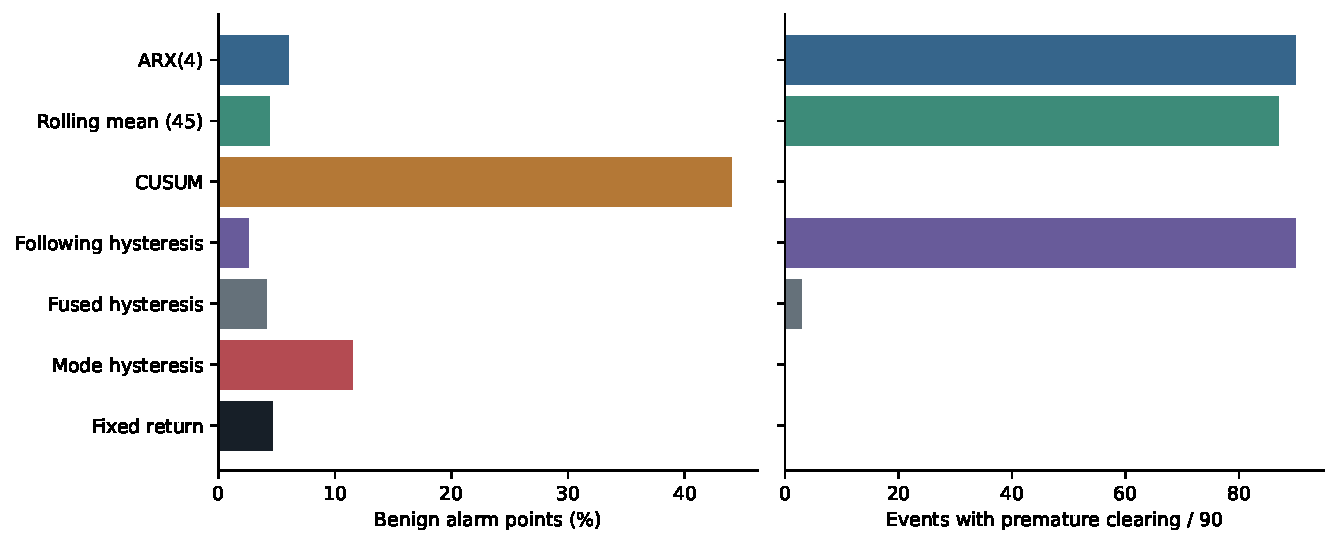
\includegraphics[width=\linewidth]{figures/tradeoff.pdf}
\caption{Benign alarm time and premature clearing describe different costs. All panels use saved pooled outcomes; zero premature clearing alone can also describe a method that remains alarmed. }
\label{fig:tradeoff}
\end{figure}

\subsection{Component ablations}
At the candidate's identical entry threshold, ordinary hysteresis had five premature-clear events, one-sample fixed return had 44, and removing the noise margin had one. The full rule had none (Table~\ref{tab:matched}). Removing the dwell reduced benign alarms from 2,778 to 1,813; removing the margin reduced them to 2,486. Both components reduced premature clearing while increasing benign alarm time.

\begin{table}[htbp]\centering\small
\caption{Matched-entry component study. All rows use $h=\CandidateThreshold$. These diagnostics do not have matched calibration alarm counts.}
\begin{tabular}{lrrr}
\toprule
Decision at same entry threshold & Benign points & Early clears & F1 \\
\midrule
Fixed return & 2778 & 0 & 0.650 \\
Matched point & 1430 & 90 & 0.731 \\
Matched hysteresis & 2389 & 5 & 0.680 \\
Matched no dwell & 1813 & 44 & 0.706 \\
Matched no margin & 2486 & 1 & 0.674 \\
\bottomrule
\end{tabular}
\label{tab:matched}
\end{table}

With separate normal-only calibration, the no-dwell variant had 1,872 benign points and 44 premature-clear events; the no-margin variant had 2,488 and one. Replacing fused entry with reference-only entry yielded 2,547 benign points and no premature clearing. Replacing it with following-only entry produced exactly the same alarm and unknown arrays as the full candidate in every one of the 144 episodes. Sample-by-sample comparison confirmed this equality. Reference-based \emph{entry} therefore added no observed decision benefit. The reference continued to supply the recovery condition.

The command-reset control and fused hysteresis had identical aggregate outcomes. Their internal state trajectories were not tested for equivalence.

\subsection{Plant conditions}
All four listed stateful methods produced zero benign alarms in P1. Fixed return produced 936 in P2 and 1,842 in P3, compared with 882 and 1,570 for fused hysteresis. Mode hysteresis produced 1,102 and 5,742. Fixed return increased benign alarm points relative to fused hysteresis in both lagged plants. Increasing model discrepancy and noise co-varied across these declared strata; the experiment does not isolate the causal effect of actuator lag from the independently changed masses, damping and sensor noise.

\begin{figure}[htbp]\centering
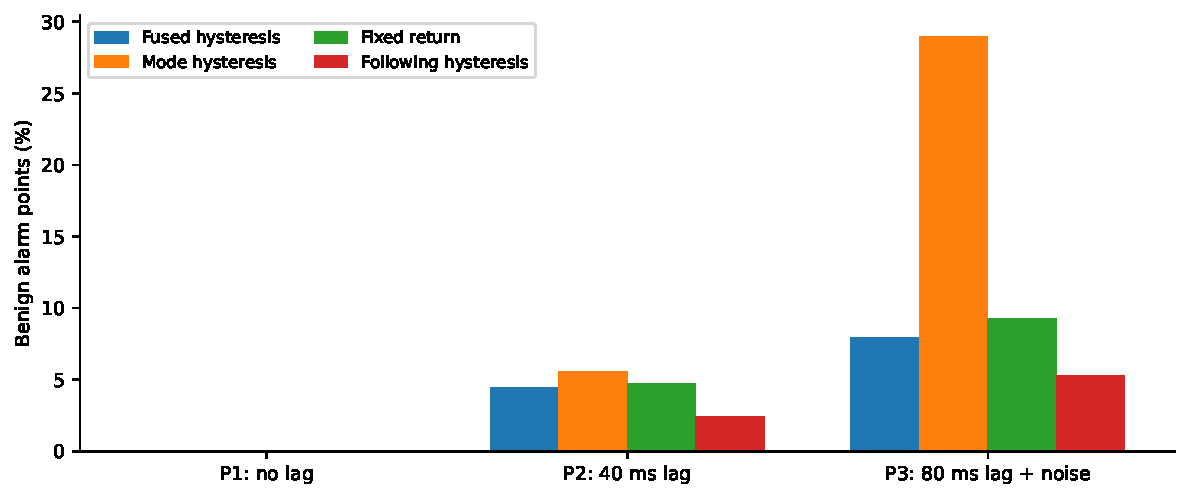
\includegraphics[width=.95\linewidth]{figures/plant_strata.pdf}
\caption{Plant-stratified benign alarm burden; each stratum contains 19,800 benign observations. Masses and damping also differ between plants, so this is not a controlled lag-only effect.}
\label{fig:strata}
\end{figure}



\subsection{Computational cost}
The supervised run completed in \Wall~s wall time and \CPU~s worker CPU time, with \RSS~MiB peak measured memory and \Output~MiB outputs. The single run completed within all resource limits. Physical generation took 17.245~s, following-observer propagation 46.921~s, shared model-bank propagation 10.073~s and score assembly 0.627~s. These are measured component totals, not independent latency estimates for each method. Model-bank work is cached across compatible episodes and includes calibration; the separately reported calibration total overlaps some of it and must not be added again.

Candidate decision replay alone took about 11.207 ms summed across all 144 saved streams, excluding prediction and scoring. Vectorized point decisions and sequential state machines have different implementation paths, so those totals are not an embedded deployment benchmark. 

\section{Discussion}
The component tests separate detection from recovery. Holding the entry threshold fixed, a ten-sample dwell reduced premature clearing from 44 events to zero, while increasing benign alarm time. Following-error hysteresis achieved the highest F1 among the selected controls, but cleared before the declared return in every event. This difference arises partly from the labels: retaining an alarm after command corruption ends lowers command-interval precision even when the robot has not yet returned to its reference trajectory.

The additional reference-based entry score provided no decision benefit in these conditions. Removing it left all alarm arrays unchanged. The reference still governed recovery, so this finding supports simplifying entry rather than discarding the reference. Fixed return also failed to improve benign alarm burden relative to fused hysteresis in either lagged plant. Its favorable result in earlier development did not extend to the new task and plant settings.

\subsection{Limitations}
Recovery was defined as proximity of the true simulated state to a nominal reference. This is a diagnostic tolerance, not a measured safe set or production-quality requirement. The reference is itself affected by model mismatch. Gaussian noise is unbounded, and the three-model envelope does not guarantee containment of all possible trajectories. Zero observed premature clears consequently provides no safety guarantee.

The study covers two analytic tasks and three plant settings within one simulator. Noise seeds repeat the same deterministic physical trajectories, and masses, damping, lag and noise co-vary between settings. The results do not isolate the effect of each physical parameter or establish performance across robots. The assumed protected command channel and truthful sensors also exclude attacks that compromise both sources.

Independent simulations and public recordings could test how far these findings extend. For example, voraus-AD provides robot fault observations \cite{voraus}, but its target signals would need a separate trust assessment before use as approved commands. Fault labels would also support a different evaluation from the present command-corruption and recovery task. Any redesign informed by these results requires newly reserved conditions for confirmation.

\section{Conclusion}
Fixed-return alarm logic eliminated observed premature clearing in the specified simulation, but increased benign alarm points by \RelativeIncrease\% relative to fused hysteresis and failed the predeclared improvement target. The matched-threshold ablations identify the recovery dwell as a useful component; reference-based entry added no decision benefit. The remaining problem is to retain reliable recovery evidence without prolonging alarms caused by legitimate motion and model mismatch.

\clearpage
\appendix
\section{Complete performance roster}\label{app:all}
IDs are stable across every table. IDs 18--21 are the matched-entry diagnostic track; other methods use the declared normal-budget calibration. Precision/recall/F1 are command-interval metrics; AP uses the underlying score and is insensitive to alternative latches sharing that score.
\begin{center}\small\begin{tabular}{rlrrrr}
\toprule
ID & Method & Precision & Recall & F1 & AP \\
\midrule
0 & Persistence & 0.187 & 0.044 & 0.071 & 0.099 \\
1 & AR(4) & 0.179 & 0.057 & 0.087 & 0.131 \\
2 & ARX(4) & 0.516 & 0.855 & 0.644 & 0.590 \\
3 & Following observer & 0.549 & 0.921 & 0.688 & 0.908 \\
4 & Rolling mean (45) & 0.577 & 0.918 & 0.709 & 0.767 \\
5 & CUSUM & 0.123 & 0.894 & 0.216 & 0.098 \\
6 & Fused point & 0.586 & 0.920 & 0.716 & 0.835 \\
7 & Fused hysteresis & 0.536 & 0.920 & 0.677 & 0.835 \\
8 & Mode hysteresis & 0.362 & 0.920 & 0.519 & 0.836 \\
9 & Envelope point & 0.238 & 0.921 & 0.378 & 0.804 \\
10 & Envelope hysteresis & 0.142 & 0.923 & 0.246 & 0.804 \\
11 & Fixed return & 0.502 & 0.920 & 0.650 & 0.835 \\
12 & Envelope + fixed return & 0.182 & 0.922 & 0.304 & 0.804 \\
13 & No dwell & 0.569 & 0.920 & 0.703 & 0.835 \\
14 & No noise margin & 0.531 & 0.920 & 0.674 & 0.835 \\
15 & Reference entry only & 0.506 & 0.918 & 0.653 & 0.621 \\
16 & Command reset & 0.536 & 0.920 & 0.677 & 0.835 \\
17 & Following hysteresis & 0.701 & 0.920 & 0.795 & 0.908 \\
18 & Matched point & 0.607 & 0.920 & 0.731 & 0.835 \\
19 & Matched hysteresis & 0.539 & 0.920 & 0.680 & 0.835 \\
20 & Matched no dwell & 0.573 & 0.920 & 0.706 & 0.835 \\
21 & Matched no margin & 0.531 & 0.920 & 0.674 & 0.835 \\
22 & Following entry only & 0.502 & 0.920 & 0.650 & 0.908 \\
\bottomrule
\end{tabular}
\end{center}
Context-dependent methods have 1,080 unknown observations out of 158,400 (99.318\% known coverage); persistence and AR have no unknown observations. All 90 simulated intervention events have an evaluator-defined return. 
\clearpage
\section{Alarm burden and recovery for every method}
Benign points have denominator 59,400. Overlap/fresh counts have denominator 90. ``Clear / returned'' counts detected events that clear within five seconds of return, divided by detected events with a return. It does not penalize events that cleared early; that failure appears in the early-clear column. Missing detections must also be read from overlap.
\begin{center}\small\begin{tabular}{rrrrrr}
\toprule
ID & Benign points & Episodes/h & Overlap/fresh & Early clears & Clear / returned \\
\midrule
0 & 519 & 442.4 & 81/81 & 81 & 81/81 \\
1 & 878 & 1054.5 & 90/90 & 90 & 90/90 \\
2 & 3564 & 4072.7 & 90/80 & 90 & 90/90 \\
3 & 3689 & 6072.7 & 90/72 & 90 & 90/90 \\
4 & 2632 & 118.2 & 90/72 & 87 & 90/90 \\
5 & 26165 & 27.3 & 81/39 & 0 & 0/81 \\
6 & 1685 & 357.6 & 90/72 & 89 & 90/90 \\
7 & 2452 & 136.4 & 90/72 & 3 & 90/90 \\
8 & 6844 & 530.3 & 90/72 & 0 & 90/90 \\
9 & 15029 & 13821.2 & 90/64 & 0 & 90/90 \\
10 & 30820 & 615.2 & 90/44 & 0 & 62/90 \\
11 & 2778 & 124.2 & 90/72 & 0 & 90/90 \\
12 & 22379 & 1812.1 & 90/60 & 0 & 90/90 \\
13 & 1872 & 275.8 & 90/72 & 44 & 90/90 \\
14 & 2488 & 124.2 & 90/72 & 1 & 90/90 \\
15 & 2547 & 81.8 & 90/72 & 0 & 90/90 \\
16 & 2452 & 136.4 & 90/72 & 3 & 90/90 \\
17 & 1529 & 142.4 & 90/72 & 90 & 90/90 \\
18 & 1430 & 366.7 & 90/72 & 90 & 90/90 \\
19 & 2389 & 157.6 & 90/72 & 5 & 90/90 \\
20 & 1813 & 281.8 & 90/72 & 44 & 90/90 \\
21 & 2486 & 124.2 & 90/72 & 1 & 90/90 \\
22 & 2778 & 124.2 & 90/72 & 0 & 90/90 \\
\bottomrule
\end{tabular}
\end{center}
\subsection*{Benign alarm counts by plant}
\begin{center}\small\begin{tabular}{lrrrr}
\toprule
Plant & Fused hyst. & Mode hyst. & Fixed return & Following hyst. \\
\midrule
P1 & 0 & 0 & 0 & 0 \\
P2 & 882 & 1102 & 936 & 483 \\
P3 & 1570 & 5742 & 1842 & 1046 \\
\bottomrule
\end{tabular}
\end{center}
Each plant stratum has 19,800 benign targets. Complete 92-row plant/method results and all 3,312 event/episode outcomes are retained in the reproducibility package.
\clearpage
\section{Delay accounting}
Delays below are conditional on the overlap or fresh-onset subset; their omitted events are explicitly counted as ``Miss / no fresh.'' All values are seconds relative to scheduled onset or the declared physical return. A zero clearing delay can mean the method had already cleared prematurely. CUSUM has no valid clearing delay in the five-second search window.
\begin{center}\small\begin{tabular}{rrrrr}
\toprule
ID & Miss / no fresh & Overlap delay med/max (s) & Fresh delay med/max (s) & Clear max (s) \\
\midrule
0 & 9/9 & 0.02/0.06 & 0.02/0.06 & 0.00 \\
1 & 0/0 & 0.02/0.04 & 0.02/0.04 & 0.00 \\
2 & 0/10 & 0.02/1.20 & 0.02/3.68 & 0.00 \\
3 & 0/18 & 0.02/1.20 & 0.02/0.04 & 0.04 \\
4 & 0/18 & 0.04/1.20 & 0.02/0.06 & 0.02 \\
5 & 9/51 & 0.26/1.20 & 0.26/0.28 & -- \\
6 & 0/18 & 0.02/1.20 & 0.02/0.04 & 0.00 \\
7 & 0/18 & 0.02/1.20 & 0.02/0.04 & 0.20 \\
8 & 0/18 & 0.02/1.20 & 0.02/0.04 & 1.50 \\
9 & 0/26 & 0.02/1.20 & 0.02/0.02 & 1.98 \\
10 & 0/46 & 0.02/1.20 & 0.02/0.02 & 4.68 \\
11 & 0/18 & 0.02/1.20 & 0.02/0.04 & 0.92 \\
12 & 0/30 & 0.02/1.20 & 0.02/0.02 & 4.70 \\
13 & 0/18 & 0.02/1.20 & 0.02/0.04 & 0.08 \\
14 & 0/18 & 0.02/1.20 & 0.02/0.04 & 0.80 \\
15 & 0/18 & 0.02/1.20 & 0.02/0.06 & 0.92 \\
16 & 0/18 & 0.02/1.20 & 0.02/0.04 & 0.20 \\
17 & 0/18 & 0.02/1.20 & 0.02/0.04 & 0.00 \\
18 & 0/18 & 0.02/1.20 & 0.02/0.04 & 0.00 \\
19 & 0/18 & 0.02/1.20 & 0.02/0.04 & 0.18 \\
20 & 0/18 & 0.02/1.20 & 0.02/0.04 & 0.08 \\
21 & 0/18 & 0.02/1.20 & 0.02/0.04 & 0.80 \\
22 & 0/18 & 0.02/1.20 & 0.02/0.04 & 0.92 \\
\bottomrule
\end{tabular}
\end{center}
For the candidate, the maximum overlap delay is 1.20 s and the maximum fresh-onset delay is 0.04 s. The difference is caused by the missing-context cases, which have overlap but no counted fresh onset. 
\clearpage
\section{Thresholds and computation}
All thresholds were fixed before fresh generation. The calibration population contains 16,200 eligible targets; the budget ceiling is 162 alarms. Different state machines can produce different attainable counts at their smallest feasible threshold. The matched-entry diagnostic counts are intentionally not equalized.
\begin{center}\small\begin{tabular}{rrrl}
\toprule
ID & Entry threshold & Calibration alarms & Threshold source \\
\midrule
0 & 0.005089627 & 162 & Retained \\
1 & 0.001808963 & 162 & Retained \\
2 & 0.001314602 & 162 & Retained \\
3 & 0.0003537666 & 162 & Retained \\
4 & 0.00039415 & 162 & Retained \\
5 & 287.1492 & 162 & Retained \\
6 & 26.31569 & 162 & Retained \\
7 & 36.51783 & 155 & Retained \\
8 & 1.660009 & 161 & Retained \\
9 & 2.45691 & 162 & Retained \\
10 & 3.249763 & 159 & Retained \\
11 & 40.81854 & 153 & Retained \\
12 & 3.208293 & 160 & Retained \\
13 & 33.25251 & 158 & Old normal only \\
14 & 36.80601 & 160 & Old normal only \\
15 & 36.39645 & 160 & Old normal only \\
16 & 36.51783 & 155 & Old normal only \\
17 & 0.002021316 & 156 & Old normal only \\
18 & 40.81854 & 4 & Matched ID 11 \\
19 & 40.81854 & 65 & Matched ID 11 \\
20 & 40.81854 & 44 & Matched ID 11 \\
21 & 40.81854 & 72 & Matched ID 11 \\
22 & 39.91404 & 153 & Old normal only \\
\bottomrule
\end{tabular}
\end{center}
\begin{center}\small\begin{tabular}{lr}
\toprule
Component & Measured time (s) \\
\midrule
bank propagation seconds & 10.073 \\
following seconds & 46.921 \\
normal calibration seconds & 2.705 \\
physical generation seconds & 17.245 \\
score assembly seconds & 0.627 \\
\bottomrule
\end{tabular}
\end{center}
Shared component timings overlap normal calibration and must not be summed as disjoint costs. Per-method decision-only totals appear in the generated supplementary table and JSON; prediction, reference propagation and score assembly are excluded from those totals.
\section{Reproducibility}
The archived protocol binds the scientific source files, model artifacts, calibration data and evaluation configuration by hash. Thresholds were sealed before generating evaluation observations, and all scores were sealed before computing outcomes. The package retains every episode, method, seed, threshold, failure record and resource measurement. Tables and figures are generated directly from the saved results. Fourteen synthetic tests and 14,635 post-run checks passed; the latter include score replay and separate contingency-count calculations.

\clearpage
\section*{Declarations}
\textbf{Affiliation.} Muhammad Usman: COMSATS University Islamabad, Sahiwal Campus, Pakistan. Haiqa Mushtaq's affiliation, individual author contributions, funding and competing-interest statements remain unconfirmed.

\textbf{Data and code.} The observations are synthetic. Simulation code, configurations, complete results and reporting scripts are retained in the local reproducibility package; no public release has been made.

\textbf{AI assistance.} Codex (OpenAI, GPT-6-based agent) assisted literature checks, study design, programming, experiment execution, analysis and drafting. The exact serving build is unavailable. Figures and tables were generated from saved results using Python and Matplotlib. Review and approval by both named authors remain pending.

\begin{thebibliography}{10}
\interlinepenalty=10000
\bibitem{casper} H. Kayan, R. Heartfield, O. Rana, P. Burnap, and C. Perera. CASPER: Context-Aware IoT Anomaly Detection System for Industrial Robotic Arms. \emph{ACM Transactions on Internet of Things}, 5(3), Article 18, 2024. Corrected VOR v1.1, 5 February 2025. \url{https://doi.org/10.1145/3670414}.
\bibitem{edge} H. Kayan, R. Heartfield, O. Rana, P. Burnap, and C. Perera. Real-Time Anomaly Detection for Industrial Robotic Arms Using Edge Computing. \emph{IEEE Internet of Things Journal}, 12(15):29696--29712, 2025. \url{https://doi.org/10.1109/JIOT.2025.3569780}.
\bibitem{twine} M. Iqbal, S. Suhail, S. Freudenthaler, M. Fahim, and R. Matulevičius. TWINE: ISO 23247-compliant digital twin and explainable AI framework for anomaly detection. \emph{Internet of Things}, 38:101976, 2026. \url{https://doi.org/10.1016/j.iot.2026.101976}.
\bibitem{ayankoso} S. Ayankoso, F. Gu, H. Louadah, H. Fahham, and A. Ball. Artificial-Intelligence-Based Condition Monitoring of Industrial Collaborative Robots: Detecting Anomalies and Adapting to Trajectory Changes. \emph{Machines}, 12(9):630, 2024. \url{https://doi.org/10.3390/machines12090630}.
\bibitem{meseguer} J. Meseguer, V. Puig, T. Escobet, and J. Saludes. Observer gain effect in linear interval observer-based fault detection. \emph{Journal of Process Control}, 20(8):944--956, 2010. \url{https://doi.org/10.1016/j.jprocont.2010.06.017}.
\bibitem{nist} NIST/SEMATECH. CUSUM Control Charts. \emph{e-Handbook of Statistical Methods}, section 6.3.2.3. Accessed 17 October 2026. \url{https://www.itl.nist.gov/div898/handbook/pmc/section3/pmc323.htm}.
\bibitem{rapio} I. Ahmed, A. Alharbi, J. Lu, A. Jaffar, and M. Bilal. Robust Adaptive Propagated Interval Observer for Actuator Fault Diagnosis in Underactuated AUVs. \emph{Journal of Marine Science and Engineering}, 14(15):1445, 2026. \url{https://doi.org/10.3390/jmse14151445}.
\bibitem{kaisar} H. Kaisar, M. Rehan, I. Ahmed, M. Bilal, and M. Khalid. A Digital Twin-Based Cybersecurity Architecture for FDI Anomaly Detection and Isolation in Next Generation Robotic Vehicles. \emph{IEEE Open Journal of the Communications Society}, 7:12709--12728, 2026. \url{https://doi.org/10.1109/OJCOMS.2026.3739185}.
\bibitem{voraus} J. T. Brockmann, M. Rudolph, B. Rosenhahn, and B. Wandt. The voraus-AD Dataset for Anomaly Detection in Robot Applications. arXiv:2311.04765, 2023. \url{https://arxiv.org/abs/2311.04765}.
\end{thebibliography}

\end{document}
